\documentclass{../../template/tp}
\usepackage[utf8x]{inputenc}

\usepackage[frenchb]{babel}
\usepackage[T1]{fontenc}

\usepackage{charter}

\usepackage{graphicx}
\graphicspath{{figures/}}
\usepackage{amssymb}
\usepackage{amsmath}
\usepackage{wasysym} %smiley
\usepackage{hyperref}% hyperliens
\usepackage{tikz}
\usetikzlibrary{babel,positioning,calc}
\usepackage[]{circuitikz}
\usepackage{textcomp}
% \usepackage{minted}
\usepackage[long]{datetime}
\usepackage{gensymb} % \ohm, celsius
\usepackage{framed}
\usepackage{pdfpages}
\usepackage{todonotes}
\usepackage{enumitem}
\usepackage{ marvosym }
\usepackage{fancyhdr}
\usepackage{mathastext} % math as standfard text : units are respecting typography conventions.
\usepackage{siunitx}

\newcommand{\version}{1.0.2}

% \langexam{frenchb}

\newboolean{koriG}
\ifx\koriG\undefined
\correction{false}
\else
\correction{true}
\fi

% \correction{false}
% \correction{true}

%% fancy header & foot
\pagestyle{fancy}
\lhead{[EL3T] Électronique appliquée\\ Exercices : BJT\ifthenelse{\boolean{corrige}}{~-- Corrigé}{}}
\rhead{v\version\\ page \thepage}
\cfoot{}
%%

\pdfinfo{
/Author (GEI)
/ModDate (D:\pdfdate)

}
\hypersetup{
pdfauthor={GEI},
pdfsubject={BJT}
}

\newcommand{\itgv}[1]{\ifthenelse{\boolean{corrige}}{\color{blue}#1}{}} %si corrigé vrai...
\newcommand{\ifgv}[1]{\ifthenelse{\boolean{corrige}}{}{#1}} %si corrigé faux...

\setlength{\parskip}{0.4cm plus4mm minus1mm} %espacement entre §
\setlength{\parindent}{0pt}

\author{GEI}

\begin{document}

\tptitle{}{Exercices : BJT}
% \thispagestyle{empty}




\Question{
    Donnez les courants et tensions de chaque branche des montages suivants, en supposant que $V_{BE} = 0.7 V$ et que $I_B \ll I_C$.
    \begin{center}
        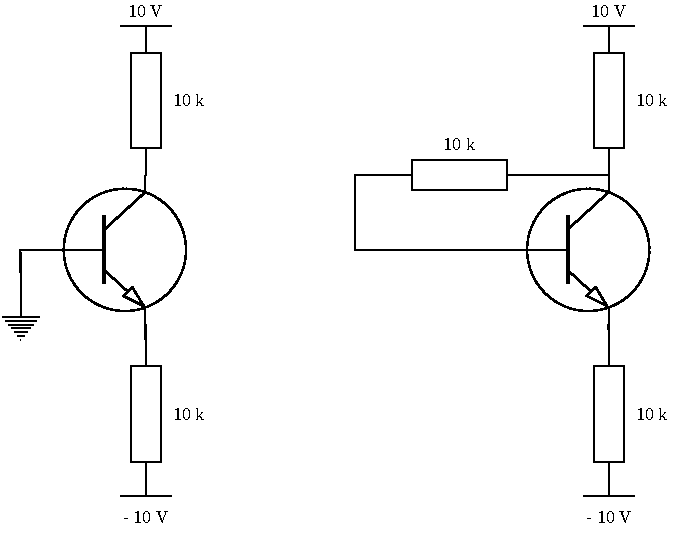
\includegraphics[width=.6\textwidth]{NPN-a.pdf}
    \end{center}
}
{
De gauche à droite :
\begin{enumerate}
    \item $-10 V + I_E \cdot 10k\Omega + V_{BE} = 0 \Leftrightarrow = 930 \mu A$

    $I_C = I_E$

    $ 10 V - I_C \cdot 10k\Omega - V_{CE} - 10k\Omega \cdot I_E + 10V = 0 \Leftrightarrow V_{CE} = 1.4 V$

    \item Si $I_R$ est le courant circulant dans la résistance connectée entre le $10 V$ et le collecteur, on a $I_R = I_C + I_B \approx I_C$ si $I_B$ est négligeable.
    De plus, toujours si $I_B$ est négligeable, la chute de potentiel sur la résistance connectée à la base est négligeable et $V_{BE} = V_{CE} = 0.7 V$.

    On a alors $10 V - I_R \cdot 10 k\Omega - V_{CE} - I_E \cdot 10 k\Omega + 10 V = 0$. Puisque $I_E = I_C$ et $I_R = I_C$ : $I_C = 965 \mu A$.
\end{enumerate}
}




\Question{
    \begin{center}
        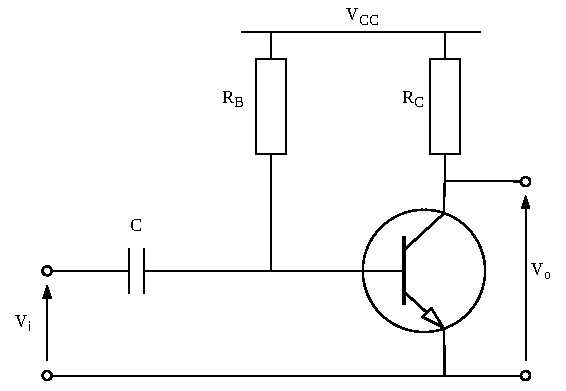
\includegraphics[]{common-emitter.pdf}
    \end{center}
    \begin{enumerate}
        \item Si $R_C = 5.6 k\Omega$, $R_B = 1 M\Omega$, $V_{CC}= 10V$, $h_{FE} = 100$, $V_{BE} = 0.7V$, que vallent $I_C$ et $V_o$ en polarisation (au repos) ?
        \item Si $h_{FE} = 500$ ?
        \item Si $h_{FE} = 10$ ?
    \end{enumerate}
}
{
\begin{enumerate}
    \item $V_{CC} - R_B \cdot I_B - V_{BE} = 0 \Leftrightarrow I_B = 9.3 \mu A$

    $I_C = h_{FE} \cdot I_B = 930 \mu A$

    $V_{CC} - I_C \cdot R_C - V_o = 0 \Leftrightarrow V_o = 4.79 V$

    \item $I_C = h_{FE} \cdot I_B = 4.65 mA$

    $V_{CC} - I_C \cdot R_C - V_o = 0 \Leftrightarrow V_o = -16.04 V$

    Cette valeur théorique n'est néanmoins pas atteignable, le transistor va saturer sur une tension $V_{CE} > 0$. En pratique, on aura une tension $V_o$ proche de 0.

    \item $I_C = h_{FE} \cdot I_B = 93 \mu A$

    $V_{CC} - I_C \cdot R_C - V_o = 0 \Leftrightarrow V_o = 9.48 V$
\end{enumerate}

}




\Question{
    Le circuit suivant est un équivalent à petit signal d'un BJT à émetteur commun.
    Légendez les courants, tensions et composants indiqués.
    \begin{center}
        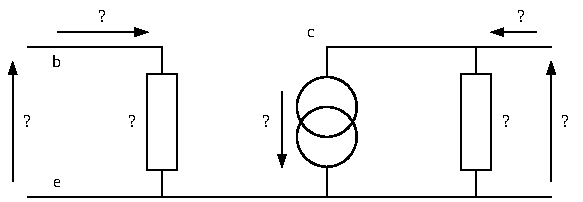
\includegraphics[]{small-signal-question.pdf}
    \end{center}
}
{
\begin{center}
    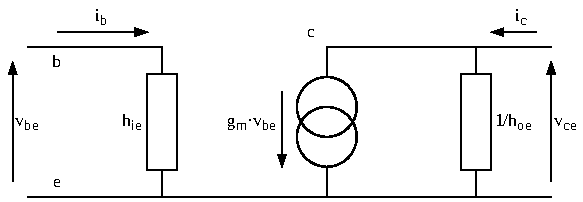
\includegraphics[]{small-signal-answer.pdf}
\end{center}
}


\Question{
    \begin{center}
        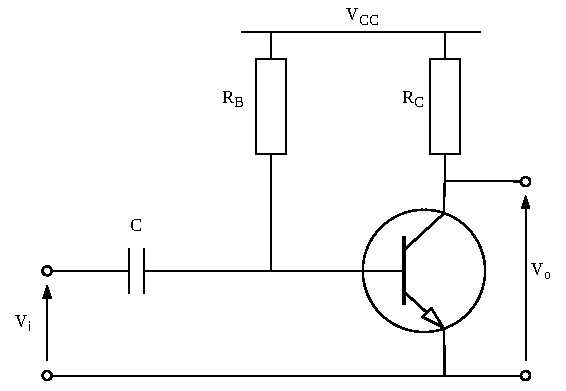
\includegraphics[]{common-emitter.pdf}
    \end{center}
    Considérons un montage à émetteur commun avec $R_C = 1 k\Omega$, $R_B = 330 k\Omega$, $V_{CC}= 12V$, $h_{FE} = 175$ et $h_{oe} = 15 \mu S$.

    \begin{itemize}
        \item Dessinez le circuit équivalent à petit signal.
        \item Calculez le gain en tension du montage à petit signal.
        \item Calculez la résistance d'entrée.
        \item Calculez la résistance de sortie.
        \item Que devient le gain du montage si une charge résistive de $1 k\Omega$ est connectée en sortie ?
    \end{itemize}
}
{

}







% \Question{
%     Dimensionnez un montage inverseur ayant un gain de \textbf{xxx} sachant que le $h_{fe}$ du transistor sélectionné vaut 200.
% }
% {

% }


\Question{
    Vous souhaitez contrôler un relais avec le montage suivant~:
    \begin{center}
        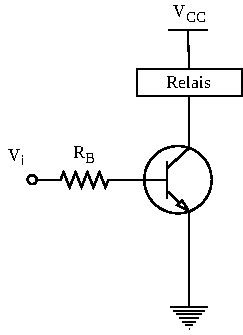
\includegraphics[]{relay.pdf}
    \end{center}
    Vous utiliez un transistor NPN \texttt{2N3903} dont le $h_{FE}$ est compris entre 50 et 150 (voir annexe).
    Le relais est un \texttt{HF140FF/005-2HS} (voir annexe).

    \begin{enumerate}
        \item Quelle tension $V_{CC}$ devez-vous utiliser avec ce relais ?
        \item Si $V_i = 3 V$, dimensionnez $R_B$ pour qu'on puisse activer le relais dans tous les cas. Pensez notamment à ce qu'il se passe si $h_{FE}$ varie dans l'intervalle indiqué.
        \item Toujours pour $V_i = 3V$, dimensionnez $R_B$ pour que le courant $I_C$ dans le transistor ne dépasse pas la valeur maximale recommandée.
    \end{enumerate}
}
{
    \begin{enumerate}
        \item $V_{CC} = 5 V$, c'est ce qu'indique la partie « 005 » de son numéro de série.
        \item Il faut dimensionner $R_B$ pour le pire cas possible. Ce dernier survient de la combinaison de deux paramètres : la tension $V_{CE}$ du transistor est nulle lorsqu'il est activé (donc $I_C$ est maximal) et $h_{FE}$ est minimal, ce qui implique que le courant $I_B$ doit être plus important pour permettre qu'un courant suffisant circule dans le relais.

        Ce dernier se comporte comme une résistance de $47 \Omega$ quand il est activé (voir datasheet, type standard et tension nominale de 5V).
        Dès lors, $I_C = V_{CC}/47\Omega = 5 V/47\Omega = 106 mA$.

        On a $I_C = h_{FE} \cdot I_B$, donc $I_B = 106mA/50 = 2.13 mA$.

        La maille d'entrée peut s'exprimer comme suit~: $V_i - R_B \cdot I_B - V_{BE} = 0$.
        En considérant $V_{BE} = 0.65 V$, on trouve $R_B = \frac{V_i - V_{BE}}{I_B} = 1.103 k\Omega$.
        Cette valeur est un maximum afin qu'on ait un courant $I_B$ suffisamment important.

        \item On pourrait alors se demander pourquoi placer une résistance $R_B$ tout court, puisqu'une valeur plus faible engendre plus facilement le courant $I_C$ souhaité.
        En se penchant sur la datasheet du transistor, on remarque notamment que le courant $I_C$ a une valeur maximale recommandée. Dans notre cas, $I_{C,max} = 200 mA$.
        Cette fois-ci, le pire cas survient si $h_{FE}$ est maximal, soit $h_{FE} = 150$.
        Si $I_C = 200 mA$, $I_B = 1.33 mA$.
        En réutilisant la même maille qu'au point précédent, on trouve $R_B = 1.767 k\Omega$.
        Cette fois-ci, cette valeur est un minimum, puisqu'on souhaite \textit{limiter} le courant circulant dans le transistor.\\

        Ces deux contraintes font fi du comportement réel du transistor en supposant que sa tension $V_{CE}$ est nulle lorsqu'il est activé. En réalité, elle sera positive, impliquant que le courant $I_C$ circulant dans le relais et le transistor sera plus faible.
    \end{enumerate}
}



\Question{
    Concevez une porte logique \texttt{NOR} à l'aide de deux transistors NPN.
    \begin{center}
        \begin{tabular}{cc|c}
        A & B & Out \\ \hline
        0 & 0 & 1 \\
        0 & 1 & 0 \\
        1 & 0 & 0 \\
        1 & 1 & 0 \\
        \end{tabular}
    \end{center}

}
{
    \begin{center}
        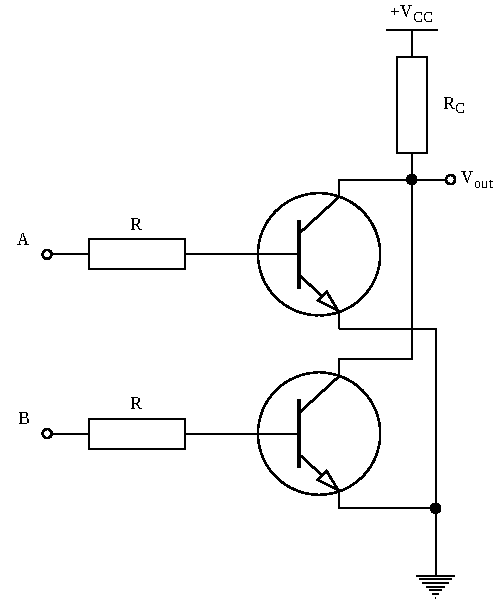
\includegraphics[]{NOR.pdf}
    \end{center}
    Le montage fonctionne grâce à une résistance $R_C$ de pull-up. Cette dernière s'assure que la tension de sortie $V_{out}$ est à l'état haut ($+ V_{CC}$) lorsque aucun courant ne circule dans la résistance.

    Si \texttt{A} et \texttt{B} sont toutes les deux à l'état bas (0 V), aucun des deux transistors n'est polarisés, donc aucune courant $I_C$ ne peut circuler, donc aucun courant ne circule dans la résistance, donc $V_{out} = V_{CC}$.

    Dès qu'une des deux entrées passe à l'état haut, le transistor correspondant est correctement polarisé, un courant $I_C$ peut alors circuler au travers du transistor et donc aussi dans la résistance, connectant la tension de sortie à la masse (en supposant que la tension $V_{CE}$ est négligeable). On a alors $V_{out} = 0 V$.
}

\Question{
    Concevez une porte logique \texttt{NAND} à l'aide de deux transistors NPN.
    \begin{center}
        \begin{tabular}{cc|c}
        A & B & Out \\ \hline
        0 & 0 & 1 \\
        0 & 1 & 1 \\
        1 & 0 & 1 \\
        1 & 1 & 0 \\
        \end{tabular}
    \end{center}

}
{
    \begin{center}
        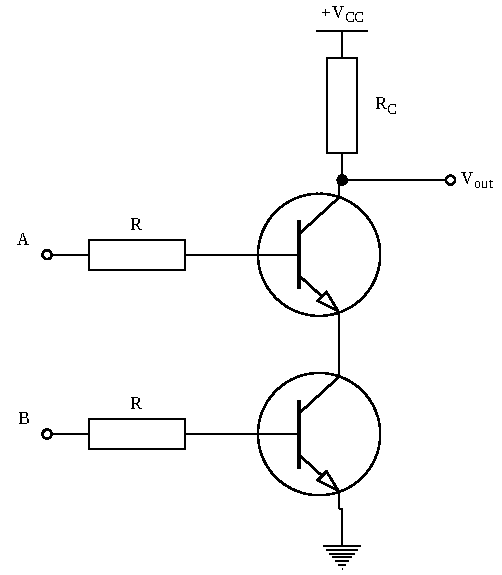
\includegraphics[]{NAND.pdf}
    \end{center}
    Le montage fonctionne grâce à une résistance $R_C$ de pull-up. Cette dernière s'assure que la tension de sortie $V_{out}$ est à l'état haut ($+ V_{CC}$) lorsque aucun courant ne circule dans la résistance.

    Le seul moyen pour qu'un courant circule dans la résistance, c'est que les deux transistors soient «~passants~», polarisés en même temps. Il faut donc que \texttt{A} \textit{et} \texttt{B} soient à l'état haut pour polariser les deux transistors en même temps et qu'un courant $I_C$ puisse s'établir dans les deux transistor, afin de connecter la tension de sortie $V_{out}$ à la masse.

    Dans tous les autres cas de figure, $V_{out} = V_{CC}$.

}
% \Question{
% }
% {}



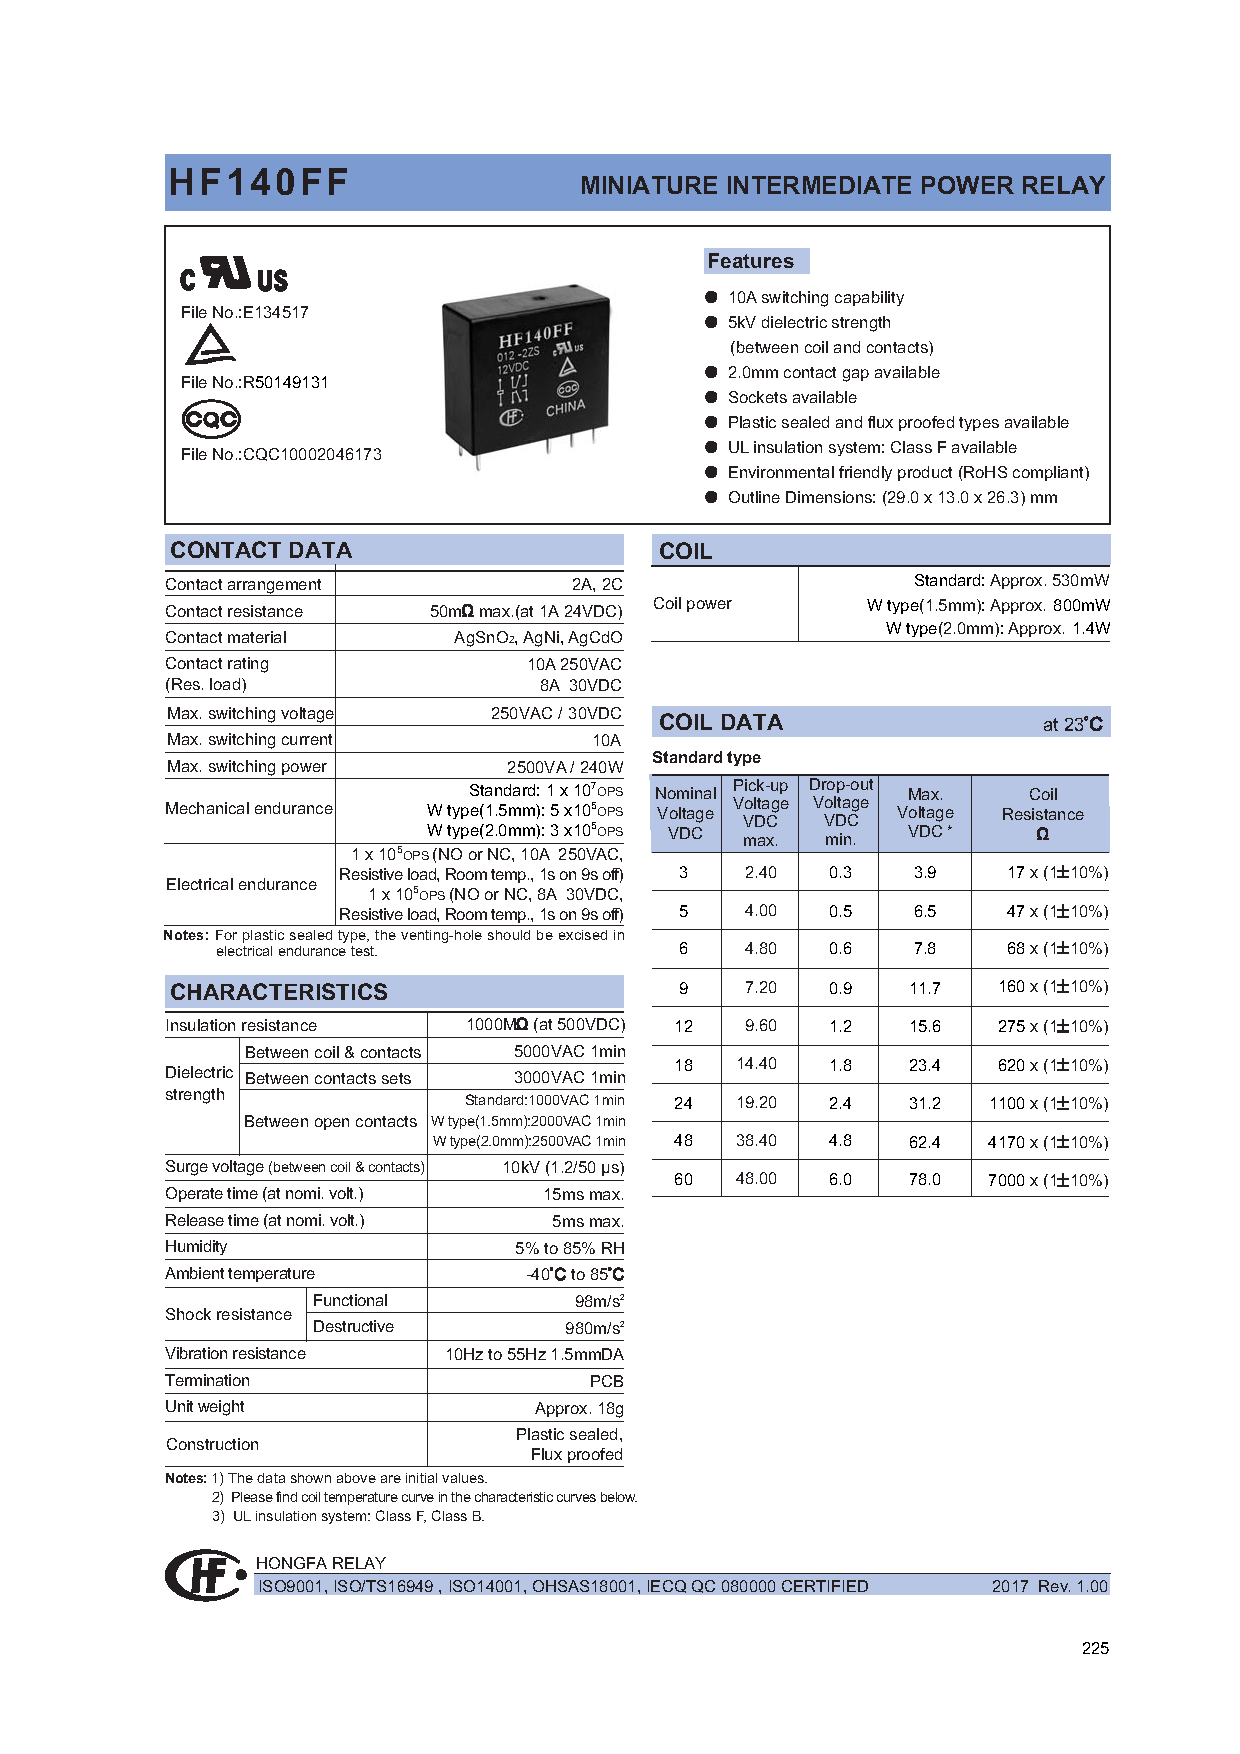
\includepdf[pages={1-3},scale=1,pagecommand={\pagestyle{plain}}]{datasheets/HF140FF.pdf}
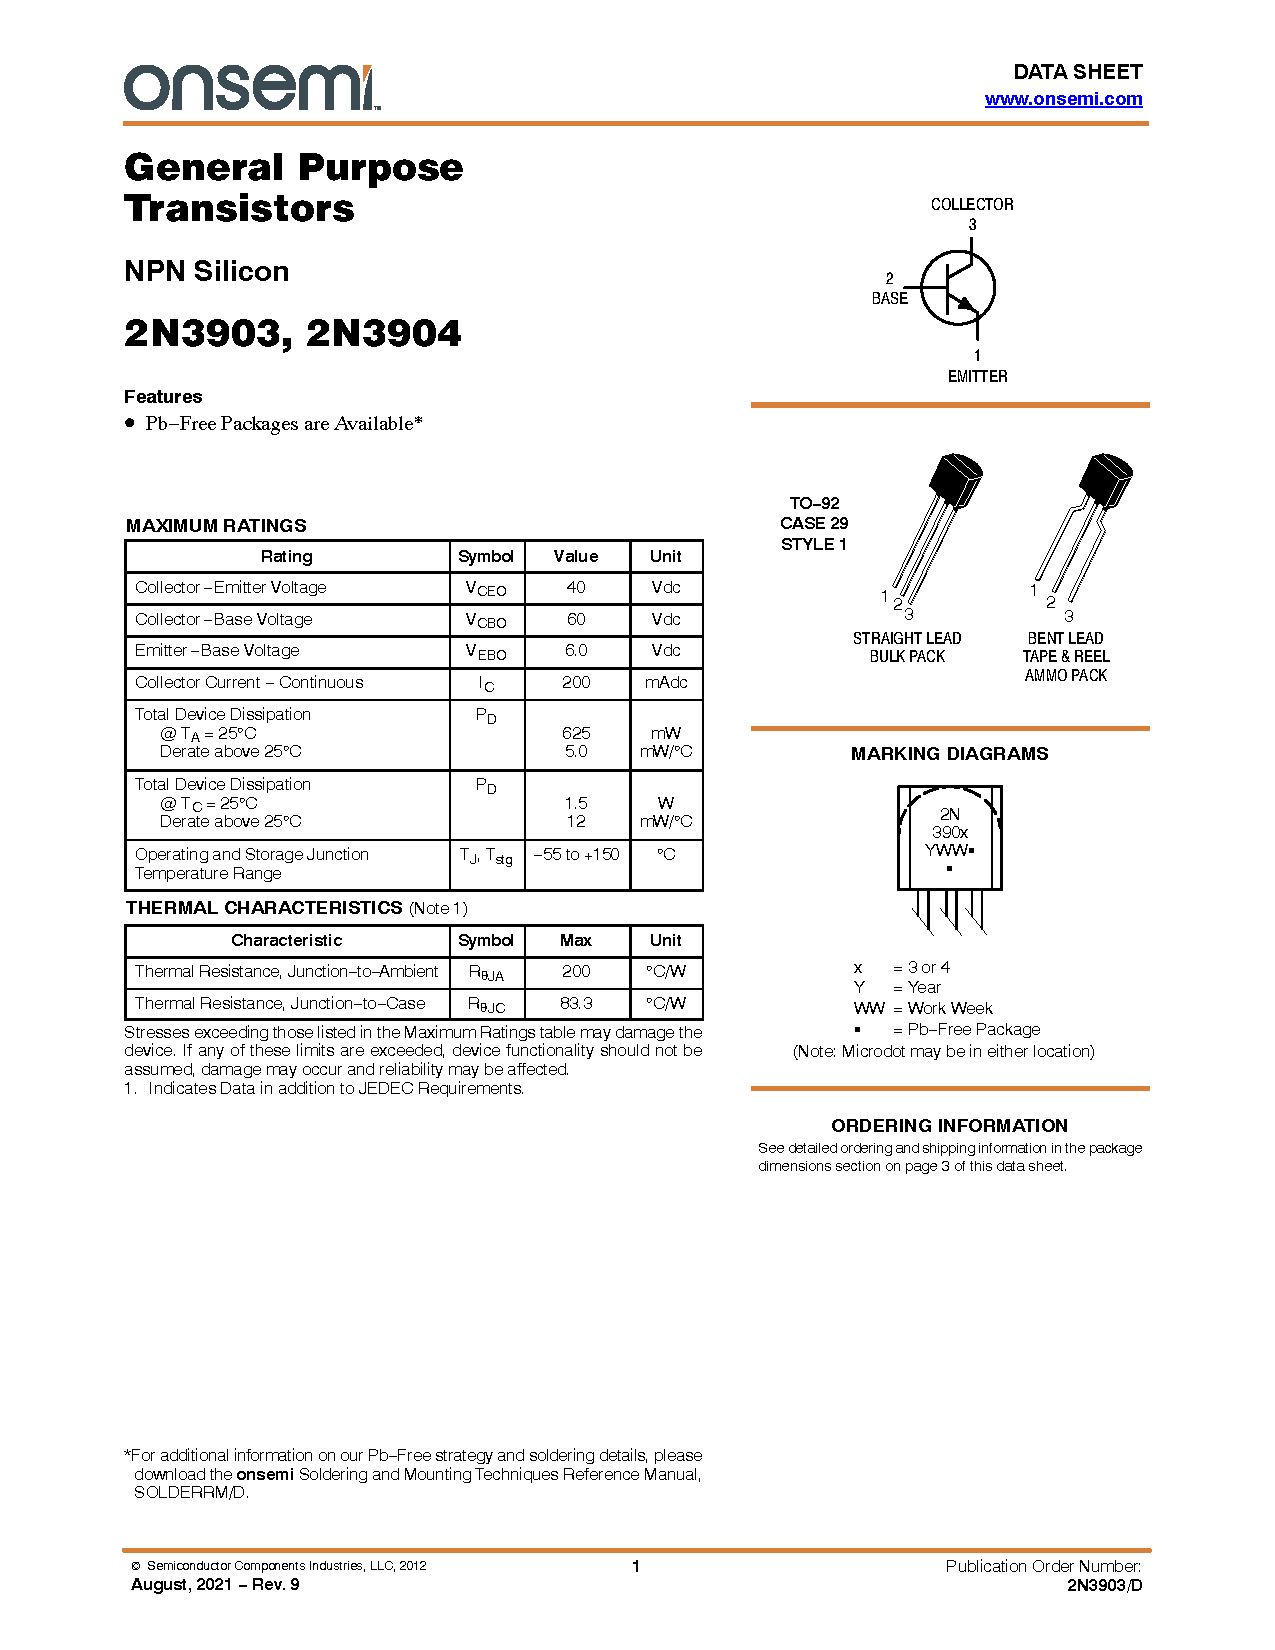
\includepdf[pages={1-2},scale=0.9,pagecommand={\pagestyle{plain}}]{datasheets/2N3903-D.PDF}
\end{document}
